
\chapter{Sprint2: Management des projets et des VMs}
\section {Introduction}
L'objectif de ce chapitre est de présenter la seconde itération du cycle de vie de notre
projet. Nous allons entamer par identifier les tâches à réaliser dans le Backlog du Sprint pour
passer par la suite aux phases d'analyse et de conception. Nous finirons par exposer la phase de
réalisation de ce module.\\
Nous avons découpés ce sprint en deux parties, une pour la gestion des projets et une autre pour le management des instances de VM qui est un élément majeur de notre application.

\section{Etude fonctionnelle}
\subsection{Backlog du Sprint} 
Le Backlog du sprint dévoilé par le tableau 3.1 comprend une liste des travaux, de chaque user story, qui seront faites durant ce sprint.



\begin{table}[H]
	\begin{tabular}{|l|l|l|l|}
		\hline
		\textbf{ID}          & \textbf{User Story}                                                                                                                                                     & \textbf{Description}                                                                                                                                                     & \textbf{Esti.} \\ \hline
		\multirow{3}{*}{3.1} & \multirow{3}{*}{\begin{tabular}[c]{@{}l@{}}En tant que Team leader, je souhaite\\ consulter mes projets.\end{tabular}}                                                  & \begin{tabular}[c]{@{}l@{}}Créer la "datatable" \\ de sélection de tous \\ les projets.\end{tabular}                                                                     & 3              \\ \cline{3-4} 
		&                                                                                                                                                                         & \begin{tabular}[c]{@{}l@{}}Implémenter l'API de\\  sélection des utilisateurs.\end{tabular}                                                                              & 3              \\ \cline{3-4} 
		&                                                                                                                                                                         & Consommer l'API.                                                                                                                                                         & 3              \\ \hline
		\multirow{3}{*}{3.2} & \multirow{3}{*}{\begin{tabular}[c]{@{}l@{}}En tant que administrateur, je souhaite\\ \\ supprimer un projet.\end{tabular}}                                              & \begin{tabular}[c]{@{}l@{}}Créer la modale de \\ confirmation de\\ suppression\end{tabular}                                                                              & 2              \\ \cline{3-4} 
		&                                                                                                                                                                         & \begin{tabular}[c]{@{}l@{}}Implémenter l'API de\\  suppression d'un \\  utilisateur.\end{tabular}                                                                        & 3              \\ \cline{3-4} 
		&                                                                                                                                                                         & Consommer l'API.                                                                                                                                                         & 3              \\ \hline

\end{tabular}
\end{table}
% Please add the following required packages to your document preamble:
% \usepackage{multirow}
\begin{table}[H]
	\begin{tabular}{|l|l|l|l|}
		\hline
		\textbf{ID}          & \textbf{User Story}                                                                                                                                                     & \textbf{Description}                                                                                                                                                     & \textbf{Esti.} \\ \hline
		\multirow{3}{*}{3.3} & \multirow{3}{*}{\begin{tabular}[c]{@{}l@{}}En tant que administrateur, je souhaite \\ créer un projet.\end{tabular}}                                                    & \begin{tabular}[c]{@{}l@{}}Créer la vue de création\\  d'un projet.\end{tabular}                                                                                         & 2              \\ \cline{3-4} 
		&                                                                                                                                                                         & \begin{tabular}[c]{@{}l@{}}Générer l'API de création\\  d'un projet.\end{tabular}                                                                                        & 3              \\ \cline{3-4} 
		&                                                                                                                                                                         & Consommer l'API.                                                                                                                                                         & 3              \\ \hline
		\multirow{3}{*}{3.4} & \multirow{3}{*}{\begin{tabular}[c]{@{}l@{}}En tant que administrateur, je souhaite\\ modifier un projet.\end{tabular}}                                                  & \begin{tabular}[c]{@{}l@{}}Créer la modale de\\  modification d'un projet.\end{tabular}                                                                                  & 2              \\ \cline{3-4} 
		&                                                                                                                                                                         & \begin{tabular}[c]{@{}l@{}}Créer l'API de modification \\ d'un projet.\end{tabular}                                                                                      & 3              \\ \cline{3-4} 
		&                                                                                                                                                                         & Consommer l'API.                                                                                                                                                         & 3              \\ \hline
		\multirow{3}{*}{3.5} & \multirow{3}{*}{\begin{tabular}[c]{@{}l@{}}En tant que Team leader, je souhaite \\ ajouter un membre à mon projet.\end{tabular}}                                        & \begin{tabular}[c]{@{}l@{}}Créer la modale de\\  consultation, affectation et \\ de détachement d'un \\ membre du projet.\end{tabular}                                   & 2              \\ \cline{3-4} 
		&                                                                                                                                                                         & \begin{tabular}[c]{@{}l@{}}Créer l'API d'ajout \\ d'un membre à un projet.\end{tabular}                                                                                  & 3              \\ \cline{3-4} 
		&                                                                                                                                                                         & Consommer l'API.                                                                                                                                                         & 3              \\ \hline
		\multirow{2}{*}{3.6} & \multirow{2}{*}{\begin{tabular}[c]{@{}l@{}}En tant que Team leader, je souhaite \\ retirer un membre de mon projet.\end{tabular}}                                       & \begin{tabular}[c]{@{}l@{}}Créer l'API de retrait \\ d'un membre d'un projet.\end{tabular}                                                                               & 3              \\ \cline{3-4} 
		&                                                                                                                                                                         & Consommer l'API.                                                                                                                                                         & 3              \\ \hline
		\multirow{5}{*}{4.1} & \multirow{5}{*}{\begin{tabular}[c]{@{}l@{}}En tant que utilisateur je souhaite \\ consulter la liste des VMs.\end{tabular}}                                             & \begin{tabular}[c]{@{}l@{}}Spécifier le nom de \\ domaine de  l'application \\ auprès de Google Cloud\\   plateform.\end{tabular}                                        & 1              \\ \cline{3-4} 
		&                                                                                                                                                                         & \begin{tabular}[c]{@{}l@{}}Générer les clés nécessaires \\ pour  autoriser les requetes \\ auprès de Google Cloud\\  plateform.\end{tabular}                             & 1              \\ \cline{3-4} 
		&                                                                                                                                                                         & \begin{tabular}[c]{@{}l@{}}Créer la "datatable" de \\ sélection de toutes\\  les instances de VMs.\end{tabular}                                                          & 3              \\ \cline{3-4} 
		&                                                                                                                                                                         & \begin{tabular}[c]{@{}l@{}}Générer l'API de sélection \\ des VMs.\end{tabular}                                                                                           & 4              \\ \cline{3-4} 
		&                                                                                                                                                                         & Consommer l'API.                                                                                                                                                         & 3              \\ \hline
			\multirow{2}{*}{4.2} & \multirow{2}{*}{\begin{tabular}[c]{@{}l@{}}En tant que utilisateur je souhaite \\ orchestrer le fonctionnement des VMs.\end{tabular}}                                   & \begin{tabular}[c]{@{}l@{}}Générer l'API \\ d'orchestration de \\ fonctionnement des VMs.\end{tabular}                                                                   & 5              \\ \cline{3-4} 
		&                                                                                                                                                                         & Consommer l'API.                                                                                                                                                         & 3              \\ \hline
		\multirow{3}{*}{4.3} & \multirow{3}{*}{\begin{tabular}[c]{@{}l@{}}En tant que Team leader je souhaite \\ créer de nouvelles instances de\\  machine  virtuelle.\end{tabular}}                  & \begin{tabular}[c]{@{}l@{}}Trouver  les options \\ utilisées dans  Google\\  Cloud  plateform pour créer \\  une VM.\end{tabular}                                        & 4              \\ \cline{3-4} 
		&                                                                                                                                                                         & \begin{tabular}[c]{@{}l@{}}Implémenter l'API de \\ création d'une VM.\end{tabular}                                                                                       & 5              \\ \cline{3-4} 
		&                                                                                                                                                                         & Consommer l'API.                                                                                                                                                         & 3              \\ \hline
	\end{tabular}
\end{table}

	\begin{table}[H]
		\begin{tabular}{|l|l|l|l|}
			\hline
			\textbf{ID}          & \textbf{User Story}                                                                                                                                                     & \textbf{Description}                                                                                                                                                     & \textbf{Esti.} \\ \hline
	
	\multirow{3}{*}{4.4} & \multirow{3}{*}{\begin{tabular}[c]{@{}l@{}}En tant que administrateur, je souhaite\\ supprimer  une machine virtuelle.\end{tabular}}                                    & \begin{tabular}[c]{@{}l@{}}Créer la modale de \\ confirmation de suppression.\end{tabular}                                                                               & 2              \\ \cline{3-4} 
	&                                                                                                                                                                         & \begin{tabular}[c]{@{}l@{}}Générer l'API de\\  suppression d'une VM.\end{tabular}                                                                                        & 4              \\ \cline{3-4} 
	&                                                                                                                                                                         & Consommer l'API.                                                                                                                                                         & 4              \\ \hline
	\multirow{2}{*}{4.5} & \multirow{2}{*}{\begin{tabular}[c]{@{}l@{}}4.5 En tant que administrateur, je souhaite\\ modifier le projet d'une machine virtuelle.\end{tabular}}                      & \begin{tabular}[c]{@{}l@{}}Générer l'API de \\ modification du projet\\  d'une VM.\end{tabular}                                                                          & 3              \\ \cline{3-4} 
	&                                                                                                                                                                         & Consommer l'API.                                                                                                                                                         & 3              \\ \hline
\end{tabular}

\caption{Backlog du Sprint 2}
\label{Backlog  du Sprint 2}
\end{table}
\subsection{Diagramme de cas d'utilisation du sprint 2}
Le diagramme de cas d'utilisation du second sprint exposé par la figure 4.1 a pour but d'établir les besoins, les résultats espérés et les mission les plus prioritaires de la seconde valeur métier.\\
Tous les cas d'utilisation de ce sprint sont précédés par une opération d'authentification.
	\begin{figure}[H]
	\centering
	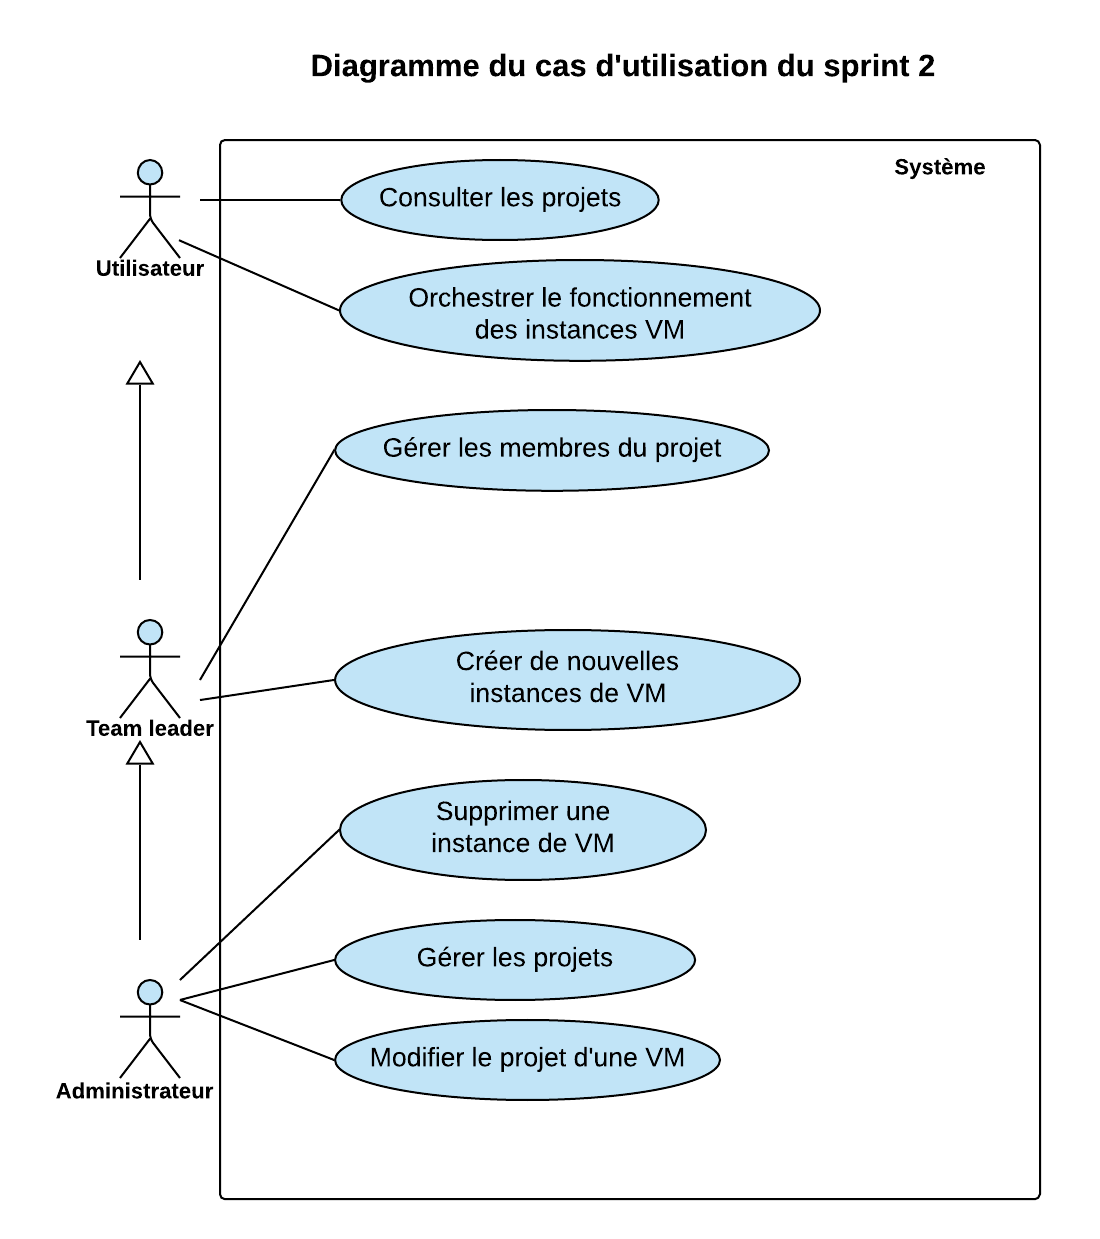
\includegraphics[scale=0.7]{DCUsprint2.png}
	\caption{Diagramme de cas d'utilisation du sprint 2}
	\label{Diagramme de cas d'utilisation du sprint 2}
\end{figure} 
Tel qu'en atteste la figure 4.1, ce sprint permet aux utilisateurs de visualiser leurs projets et les informations appropriées. Ainsi, il les permet d'orchestrer le fonctionnement des instances de machines virtuelles. Encore plus, durant cette itération, le Team leader est apte à créer de nouvelles instances de   machines virtuelles.  Quant à l'administrateur, de plus que toutes les fonctionnalités déjà citées il serait capable de gérer les projets, de créer et de supprimer les VMs non utilisées.
\section{Management des projets}
Cette section est vouée au management des projets. Celui-ci est constitué par les cas d'utilisation "gérer les projets","visualiser les projets" et "gérer les membres du projet".
\subsection{Analyse }
Pour mieux assimiler les cas d'utilisation de la première partie de ce sprint, nous allons définir, dans cette section, leurs raffinements en fournissant une description sur les scénarios.
\begin{itemize}
	\item \textbf{Raffinement du cas d'utilisation "Gérer les membres du projet"} \\
\end{itemize} 
\begin{figure}[H]
	\centering
	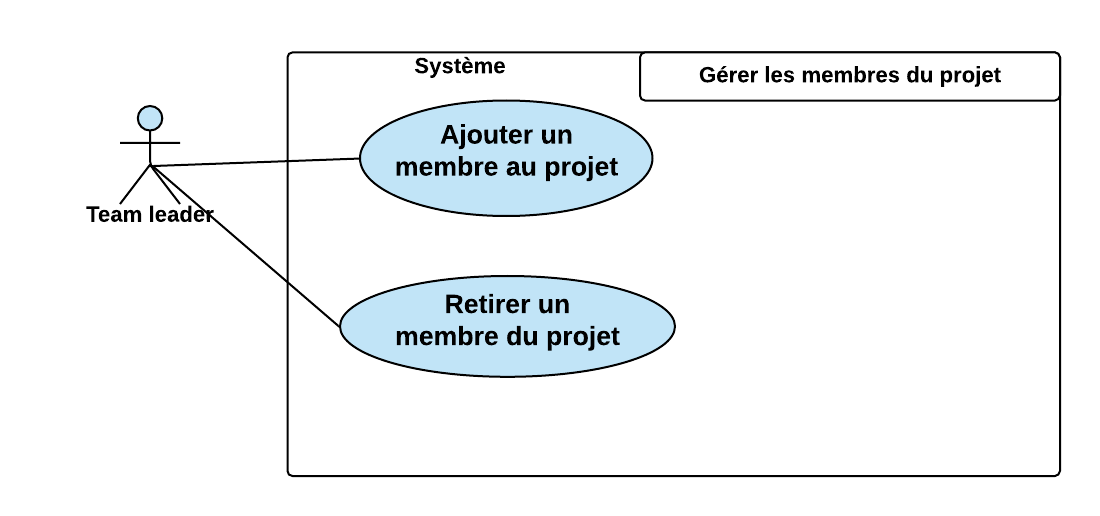
\includegraphics[ height=5cm, width=14cm]{Rgerermembre.png}
	\caption{Raffinement du cas d'utilisation: Gérer les membres du projet}
	\label{Raffinement du cas d'utilisation: Gérer les membres du projet}
\end{figure} 
% Insérer diagramme
Le diagramme de la figure 4.3 ci dessus, présente les sous cas d'utilisation qui étendent de "Gérer les membres du projet".
\subsubsection{Description textuelle du sous cas d'utilisation: "Ajouter un membre au projet"}
% Please add the following required packages to your document preamble:
% \usepackage{multirow}
\begin{table}[H]
	\begin{tabular}{|l|l|}
		\hline
		\textbf{Acteur}                               & Team leadder                                                                                                                             \\ \hline
		\textbf{Description}                          & Ajouter un nouveau membre au projet.                                                                                                    \\ \hline
		\textbf{Préconditions}                        & Team leader authentifié.                                                                                                                 \\ \hline
		\textbf{Post-conditions}                      & Membre ajouté.                                                                                                                           \\ \hline
		\multirow{4}{*}{\textbf{Scénario principal}}  & \begin{tabular}[c]{@{}l@{}}1. Le Team leader remplit les champs relatifs à l'affectation\\ d'un nouveau membre puis valide.\end{tabular} \\ \cline{2-2} 
		& 2. Le système vérifie l'existence de l'utilisateur saisit.                                                                               \\ \cline{2-2} 
		& 3. Le système enregistre le membre ajouté.                                                                                               \\ \cline{2-2} 
		& 4. Le système affiche  la liste des membres mises à jour.                                                                                \\ \hline
		\multirow{2}{*}{\textbf{Scénario altérnatif}} & \begin{tabular}[c]{@{}l@{}}1.a Le Team leader saisit un mail d'utilisateur inexistant\\  dans le système.\end{tabular}                   \\ \cline{2-2} 
		& 1.b Le système affiche un message d'erreur.                                                                                              \\ \hline
	\end{tabular}

\caption{Description textuelle du << Ajouter un membre au projet  >> }
\label{Description textuelle du << Ajouter un membre au projet >>}
\end{table}

\begin{itemize}
	\item \textbf{Raffinement du cas d'utilisation "Gérer les projets"} \\
\end{itemize} 

		\begin{figure}[H]
		\centering
		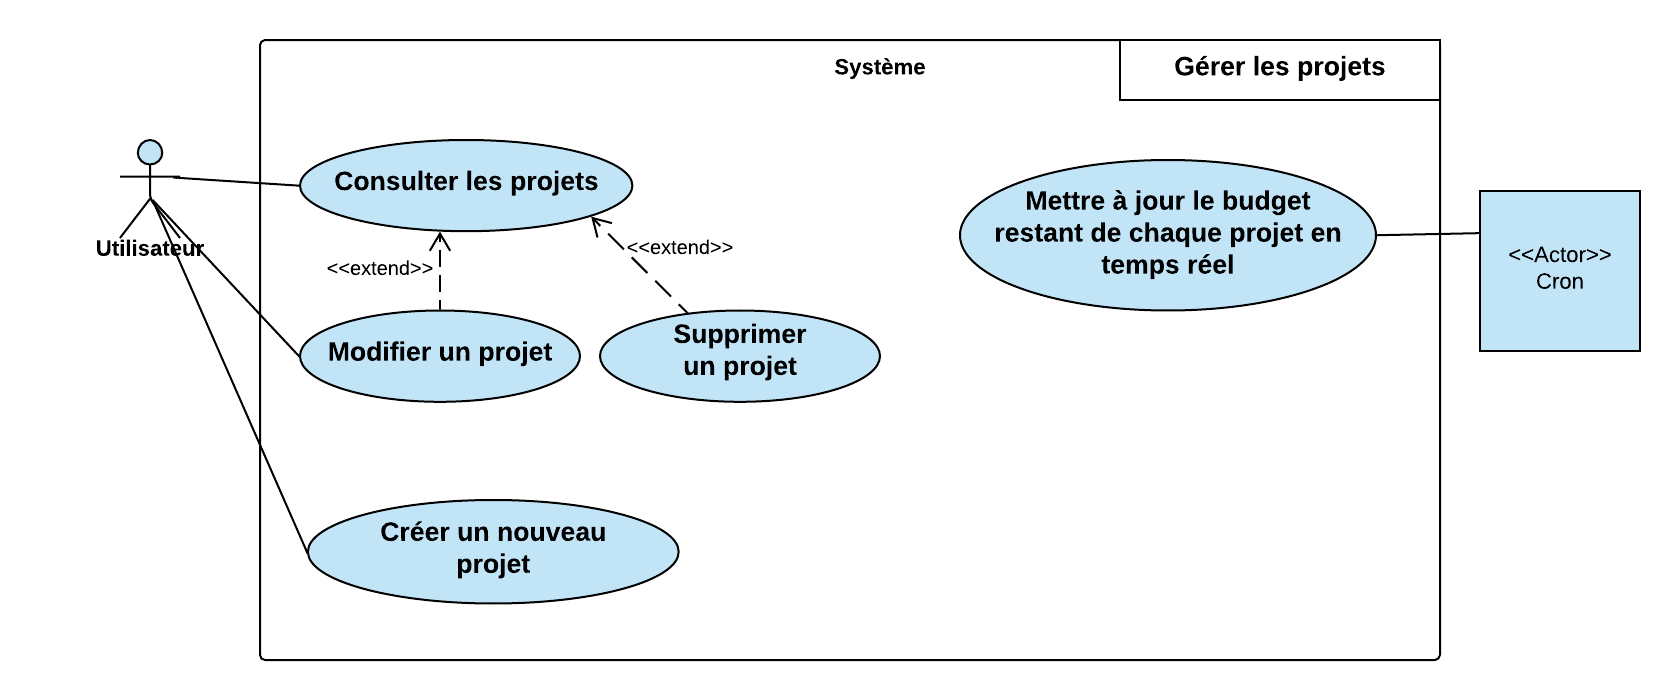
\includegraphics[ height=5.5cm, width=14cm]{Rgererprojet.png}
		\caption{Raffinement du cas d'utilisation: Gérer les projets}
		\label{Raffinement du cas d'utilisation: Gérer les projets}
	\end{figure} 
	Le diagramme de la figure 4.3 représente un raffinement relatif
au cas d'utilisation "gérer  les projets". En effet, ce cas d'utilisation fait intervenir deux acteurs. L'administrateur pour la création d'un nouveau projet et/ou  la consultation de la liste des projets et le Cron pour la mise à jour automatique  du budget restant de chaque projet. \\
En consultant la liste des projets, l'administrateur a la possibilité de modifier ou de supprimer un projet.
\subsubsection{Description textuelle du sous cas d'utilisation: "Créer un nouveau projet"}

% Please add the following required packages to your document preamble:
% \usepackage{multirow}
\begin{table}[H]
	\begin{tabular}{|l|l|}
		\hline
		\textbf{Acteur}                              & Administrateur                                                                                                                           \\ \hline
		\textbf{Description}                         & Ajouter un projet au système.                                                                                                            \\ \hline
		\textbf{Préconditions}                       & Administrateur authentifié.                                                                                                              \\ \hline
		\textbf{Post-conditions}                     & Projet créé.                                                                                                                             \\ \hline
		\multirow{3}{*}{\textbf{Scénario principal}} & \begin{tabular}[c]{@{}l@{}}1. L'administrateur remplit les champs relatifs à la création\\ d'un nouveau projet puis valide.\end{tabular} \\ \cline{2-2} 
		& 2. Le système vérifie l'unicité de projet.                                                                                               \\ \cline{2-2} 
		& 3. Le système ajoute le nouveau projet.                                                                                                  \\ \hline
		\textbf{Scénario altérnatif}                 & \begin{tabular}[c]{@{}l@{}}2.a Le système affiche un message d'erreur indiquant \\ l'existence d'un sujet pareil.\end{tabular}           \\ \hline
	\end{tabular}

\caption{Description textuelle du << Créer un nouveau projet >> }
\label{Description textuelle du << Créer un nouveau projet >>}
\end{table}


\subsection{Conception}
Dans ce qui suit, nous allons détailler et décortiquer les cas d'utilisation les plus prioritaires, de la première partie de ce sprint, à travers les diagrammes de séquences objet.
\subsubsection{Diagramme de séquence du cas d'utilisation: "Mettre à jour  le budget restant de chaque projet en temps réel"}

\begin{figure}[H]
	\centering
	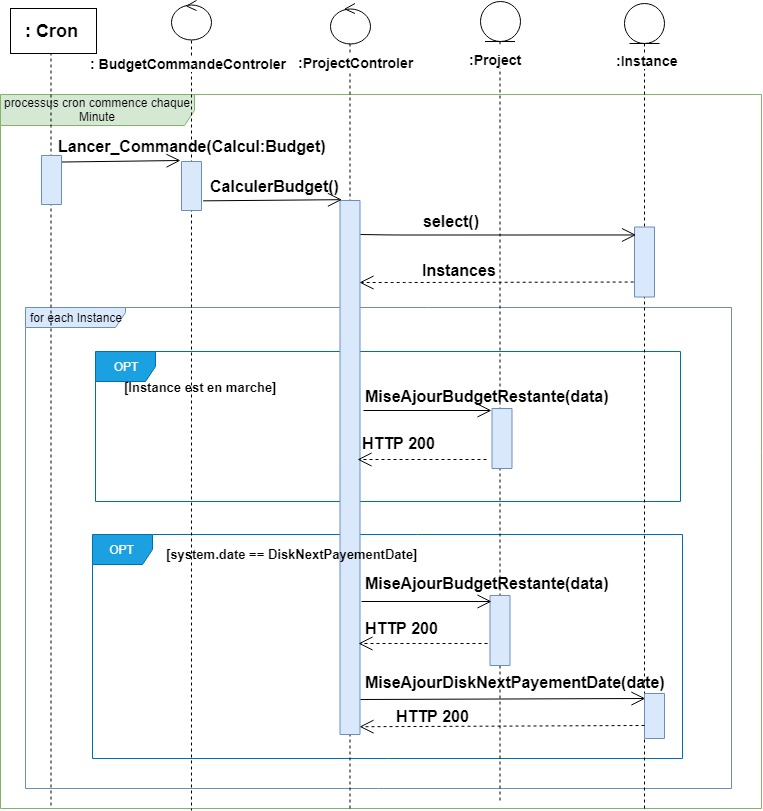
\includegraphics[scale=0.54]{budget2.jpg}
	\caption{Diagramme de séquence: Mettre à jour le budget restant du projet en temps réel }
	\label{Diagramme de séquence: Mettre à jour le budget restant du projet en temps réel }
\end{figure}
Le diagramme de la figure 4.4 détaille la procédure de mise à jour automatique du budget restant de chaque projet. Tout d'abord, Cron lance la commande responsable à la consommation de l'API permettant de calculer le budget restant. Cette opération se répète périodiquement chaque minute. En effet  
cet API consiste à sélectionner toutes les instances de VM et  de faire deux tests pour chaque instance. 
Le premier consiste à vérifier l'état de la machine, si elle est en marche. Le budget restant sera mis à jour. 
Le second consiste à vérifier les dates de système et du prochain payement. S'ils coïncident  le contrôleur  met à jour le budget restant et la date du prochain payement.  Vu que le payement du disque ne s'effectue qu'une seule fois par mois.    
\section{Management des VMs}
Cette section est vouée au management des instances de machines virtuelles qui sont une entité phare dans notre projet. Celui-ci est constitué par les cas d'utilisation "Orchestrer les instances de VM","Créer de nouvelles instances de VM" , "Supprimer une VM" et "Modifier le projet d'une VM".\\
Toutes les taches de cette partie nécessite une préalable configuration au près du Google Cloud plateform pour autoriser l'émission des requêtes à partir de notre application.
\subsection{Analyse}
Dans ce qui suit, nous allons offrir une vue d'ensemble des différentes fonctionnalités
relatives à la deuxième partie de ce sprint. Ensuite, nous allons raffiner et décrire les cas
d'utilisation les plus prioritaires.
\begin{itemize}
	\item \textbf{Raffinement du cas d'utilisation "Orchestrer les instances de VM"}
	 
		\begin{figure}[H]
		\centering
		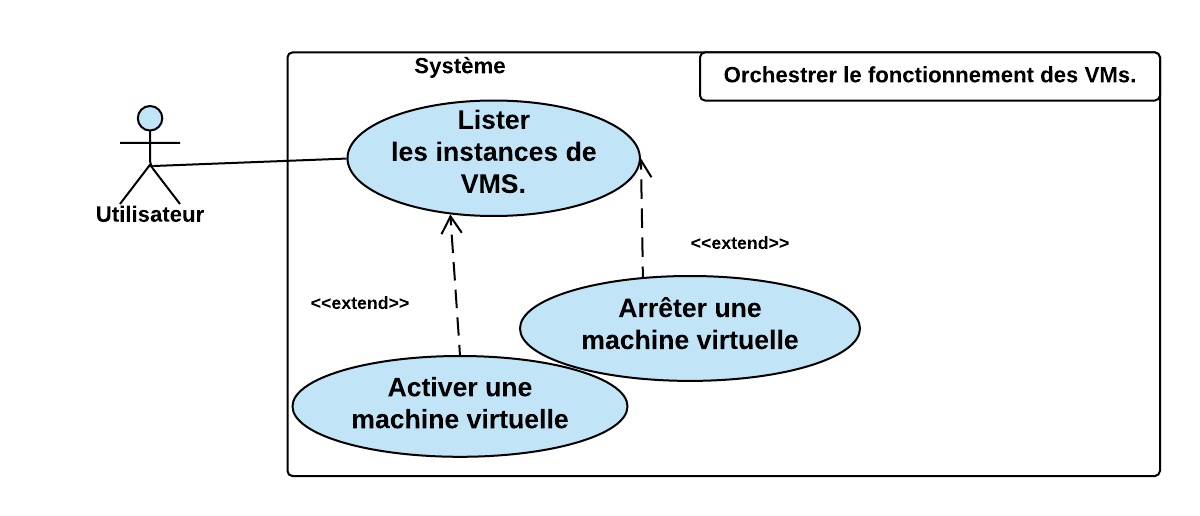
\includegraphics[ height=4cm, width=14cm]{Rorchestrer.png}
		\caption{Raffinement du cas d'utilisation: Orchestrer le fonctionnement des VMs}
		\label{Raffinement du cas d'utilisation: Orchestrer le fonctionnement des VMs}
	\end{figure} 
\end{itemize}
	Le diagramme de cas d'utilisation de la figure 4.5 met en évidence un raffinement lié
au cas d'utilisation "Orchestrer le fonctionnement des VMs". Cette opération est assurée à travers la consultation de la liste des machines virtuelles ou l'utilisateur peut  activer ou arrêter une VM.
\subsubsection{Description textuelle du cas d'utilisation: "Lister les instances de VM"}

% Please add the following required packages to your document preamble:
% \usepackage{multirow}
\begin{table}[H]
	\begin{tabular}{|l|l|}
		\hline
		\textbf{Acteur}                               & Utilisateur.                                                                                                                         \\ \hline
		\textbf{Description}                          & Récupérer les instances de VM                                                                                                        \\ \hline
		\textbf{Préconditions}                        & 1.Utilisateur authentifié.                                                                                                           \\ \hline
		\textbf{Post-conditions}                      & Liste des instances de VM récupérée.                                                                                                 \\ \hline
		\multirow{3}{*}{\textbf{Scénario principal}}  & 1. L'utilisateur demande l'accès à la liste des  instances de VM.                                                                       \\ \cline{2-2} 
		& \begin{tabular}[c]{@{}l@{}}2. Le système récupère la liste des projets auquel appartient\\ l'utilisateur courant.\end{tabular}       \\ \cline{2-2} 
		& \begin{tabular}[c]{@{}l@{}}3. Le système affiche la liste des instances de VM des projets\\ retournés\end{tabular}                   \\ \hline
		\multirow{2}{*}{\textbf{Scénario altérnatif}} & 2.a L'utilisateur n'appartient à aucun projet.                                                                                       \\ \cline{2-2} 
		& \begin{tabular}[c]{@{}l@{}}2.b Le système affiche un message indiquant que l'utilisateur\\ n'appartient à aucun projet.\end{tabular} \\ \hline
	\end{tabular}

\caption{Description textuelle du << Lister les instances de VM >> }
\label{Description textuelle du << Lister les instances de VM >>}
\end{table}

\subsubsection{Description textuelle du sous cas d'utilisation: "Activer une machine virtuelle"}
% Please add the following required packages to your document preamble:
% \usepackage{multirow}
\begin{table}[H]
	\begin{tabular}{|l|l|}
		\hline
		\textbf{Acteur}                               & Utilisateur.                                                                                                              \\ \hline
		\textbf{Description}                          & Activer une machine virtuelle.                                                                                            \\ \hline
		\multirow{2}{*}{\textbf{Préconditions}}       & 1.Utilisateur authentifié.                                                                                                \\ \cline{2-2} 
		& 2. Requetes autorisées.                                                                                                   \\ \hline
		\textbf{Post-conditions}                      & Machine virtuelle activée.                                                                                                \\ \hline
		\multirow{4}{*}{\textbf{Scénario principal}}  & 1. L'utilisateur clique sur le bouton d'activation d'une VM.                                                              \\ \cline{2-2} 
		& 2. Le système récupère le  budget restant du projet de la VM                                                              \\ \cline{2-2} 
		& \begin{tabular}[c]{@{}l@{}}3. Le système demande au serveur du Google Compute engine\\ d'activer la VM.\end{tabular}      \\ \cline{2-2} 
		& \begin{tabular}[c]{@{}l@{}}4. Le système met à jour l'état de la VM dans la base de \\ données.\end{tabular}              \\ \hline
		\multirow{2}{*}{\textbf{Scénario altérnatif}} & \begin{tabular}[c]{@{}l@{}}2.a Le budget restant du projet insuffisant pour démarrer une \\ VM.\end{tabular}              \\ \cline{2-2} 
		& \begin{tabular}[c]{@{}l@{}}2.b Le système affiche un message d'erreur indiquant \\ l'insuffisance du budget.\end{tabular} \\ \hline
	\end{tabular}

\caption{Description textuelle du << Activer une machine virtuelle >> }
\label{Description textuelle du << Activer une machine virtuelle >>}
\end{table}

\subsection{Conception}
Afin de décortiquer et détailler les cas d'utilisation précédemment cités, nous présentons dans ce qui suit les diagrammes de séquences des cas d'utilisation les plus importants
\subsubsection{Diagramme de séquence du cas d'utilisation: "Créer une nouvelle instance de VM"}

\begin{figure}[H]
	\centering
	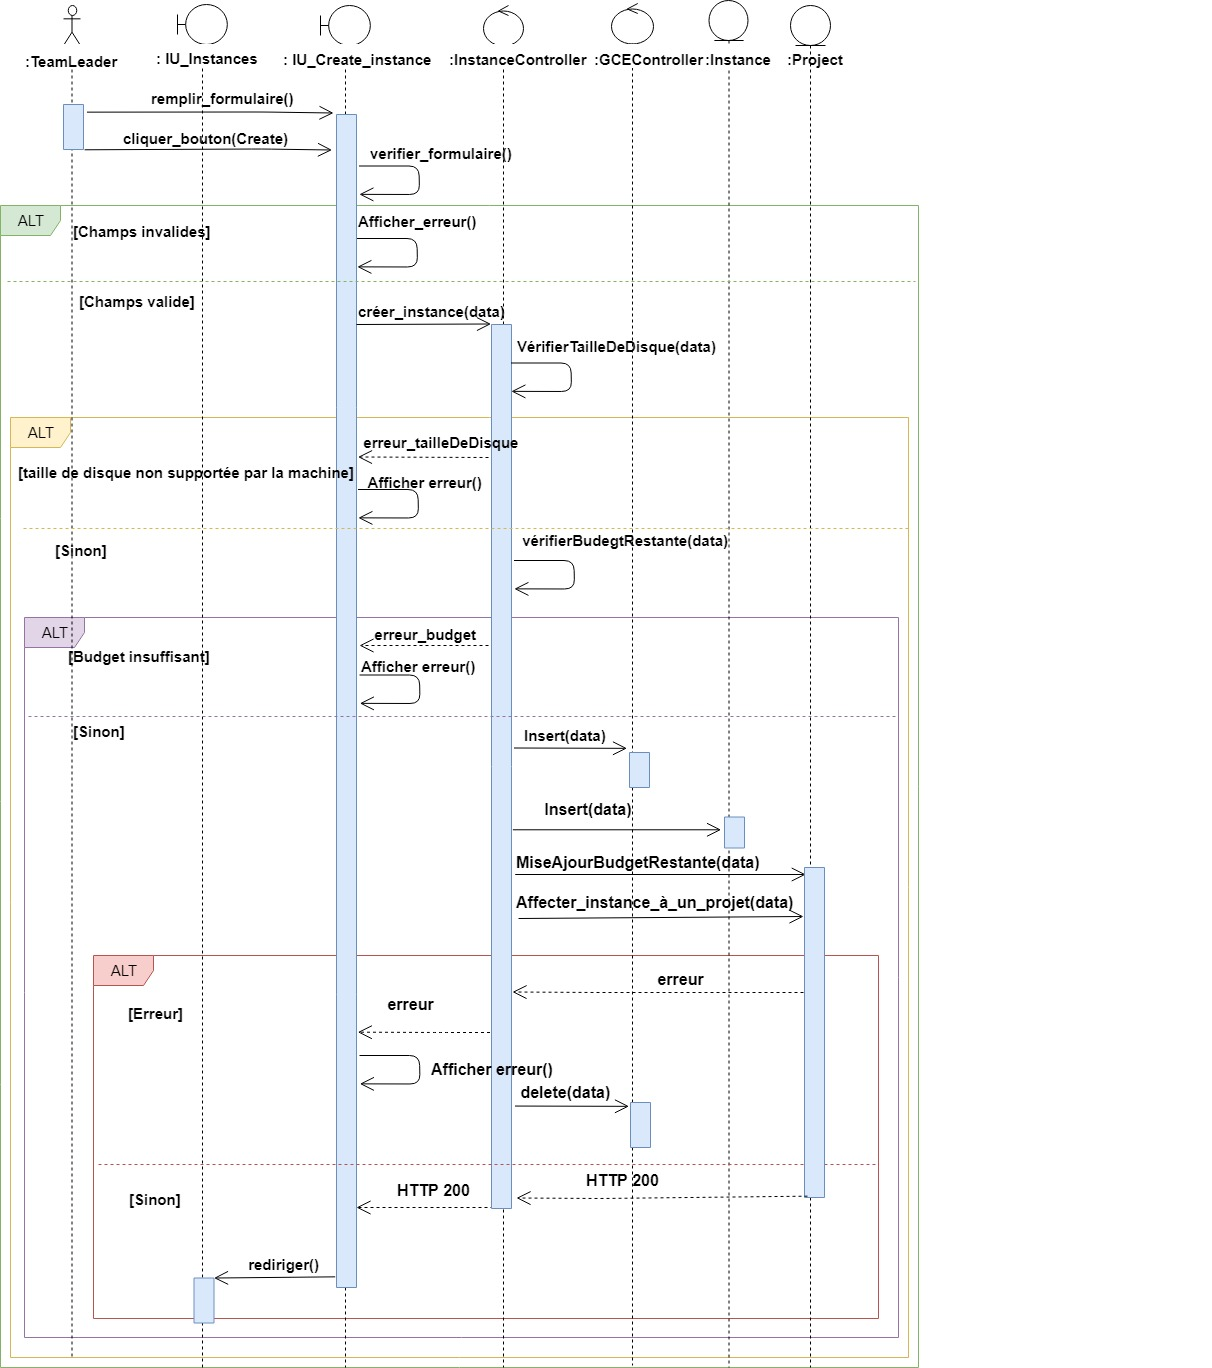
\includegraphics[ height=18cm, width=20cm]{createInstance-Page-1.jpg}
	\caption{Diagramme de séquence: Créer une nouvelle instance de VM}
	\label{Diagramme de séquence: Créer une nouvelle instance de VM}
\end{figure}
Le diagramme de la figure 4.6 illustre la procédure de création d'une instance de machine virtuelle. Tout d'abord, le Team leader remplit le formulaire  puis valide et confirme. Une fois confirmé, 
le contrôleur  vérifie la compatibilité entre la taille du disque et le type de la machine émis. S'ils sont incompatibles le contrôleur retourne une erreur, sinon il vérifie le budget restant du projet. S'il est suffisant pour créer une VM le contrôleur demande au serveur du Google Compute Engine de créer la VM puis il l'insère dans l'entité Instance et met à jour le projet associé et son budget restant. Dans le cas ou une erreur s'est produite au niveau de l'insertion dans la base de données, le contrôleur annule l'opération en supprimant la VM de la part de Google Compute Engine afin d'assurer la synchronisation.

\subsubsection{Diagramme de séquence du cas d'utilisation: "Modifier le projet d'une machine virtuelle"}

\begin{figure}[H]
	\centering
	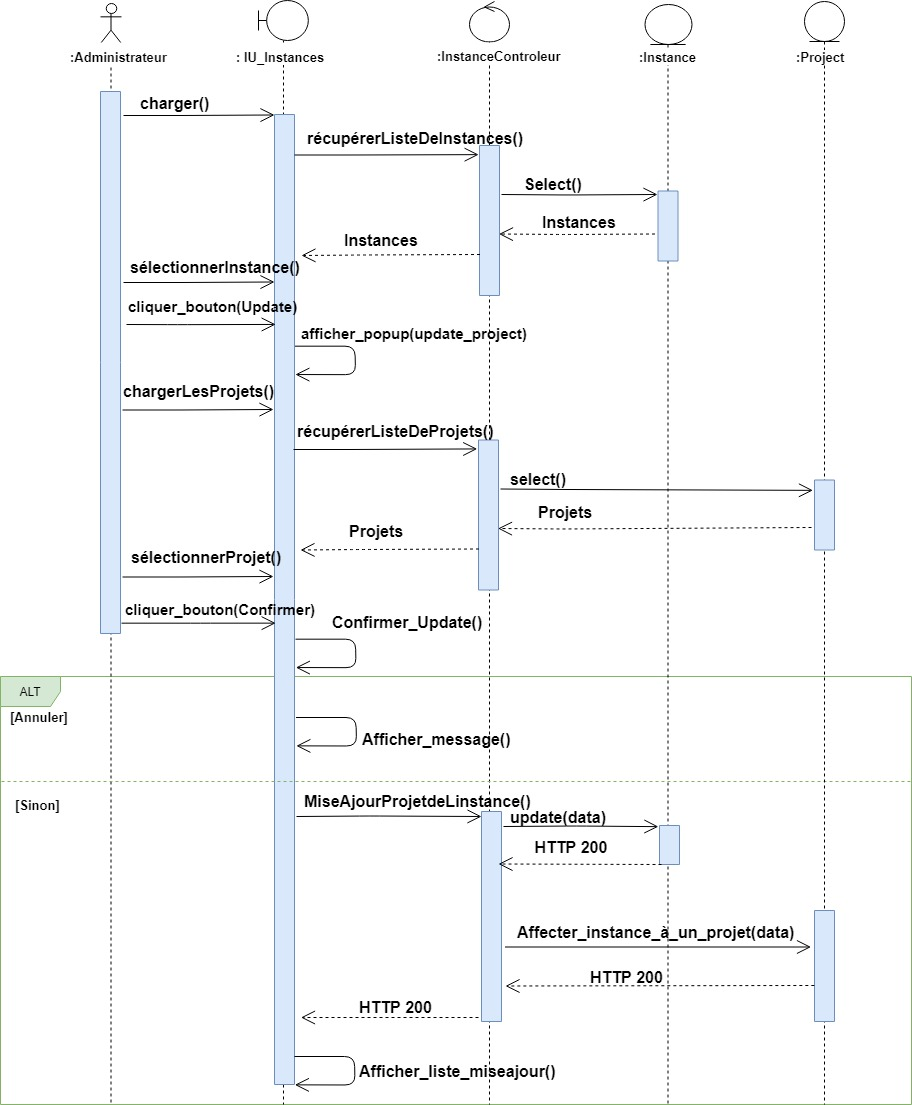
\includegraphics[scale=0.4]{updateProjectOfisntate.jpg}}
	\caption{Diagramme de séquence: Modifier le projet d'une machine virtuelle }
	\label{Diagramme de séquence: Modifier le projet d'une machine virtuelle }
\end{figure}

Le diagramme de la figure 3.8 décrit l'opération de modification du projet d'une machine virtuelle. Tout
d'abord, l'administrateur récupère toutes les instances de machine virtuelle. Ensuite, Il sélectionne la machine virtuelle adéquate et choisit le  nouveau projet  puis valide. Une fois validé, une modale de confirmation s'ouvre. Là ou
il peut soit annuler l'opération, soit la confirmer. S'il confirme 
les données nécessaires à la modification seront émises au contrôleur des instances pour effectuer les changements dans les entités Instance et projet. Finalement le contrôleur retourne une requête Htp de
statut 200 en cas de succès.

\section{Réalisation}
Passons à la partie réalisation, nous allons capturer quelques interfaces de ce deuxième 
sprint.
\subsection{Interfaces}
	\begin{figure}[H]
	\centering
	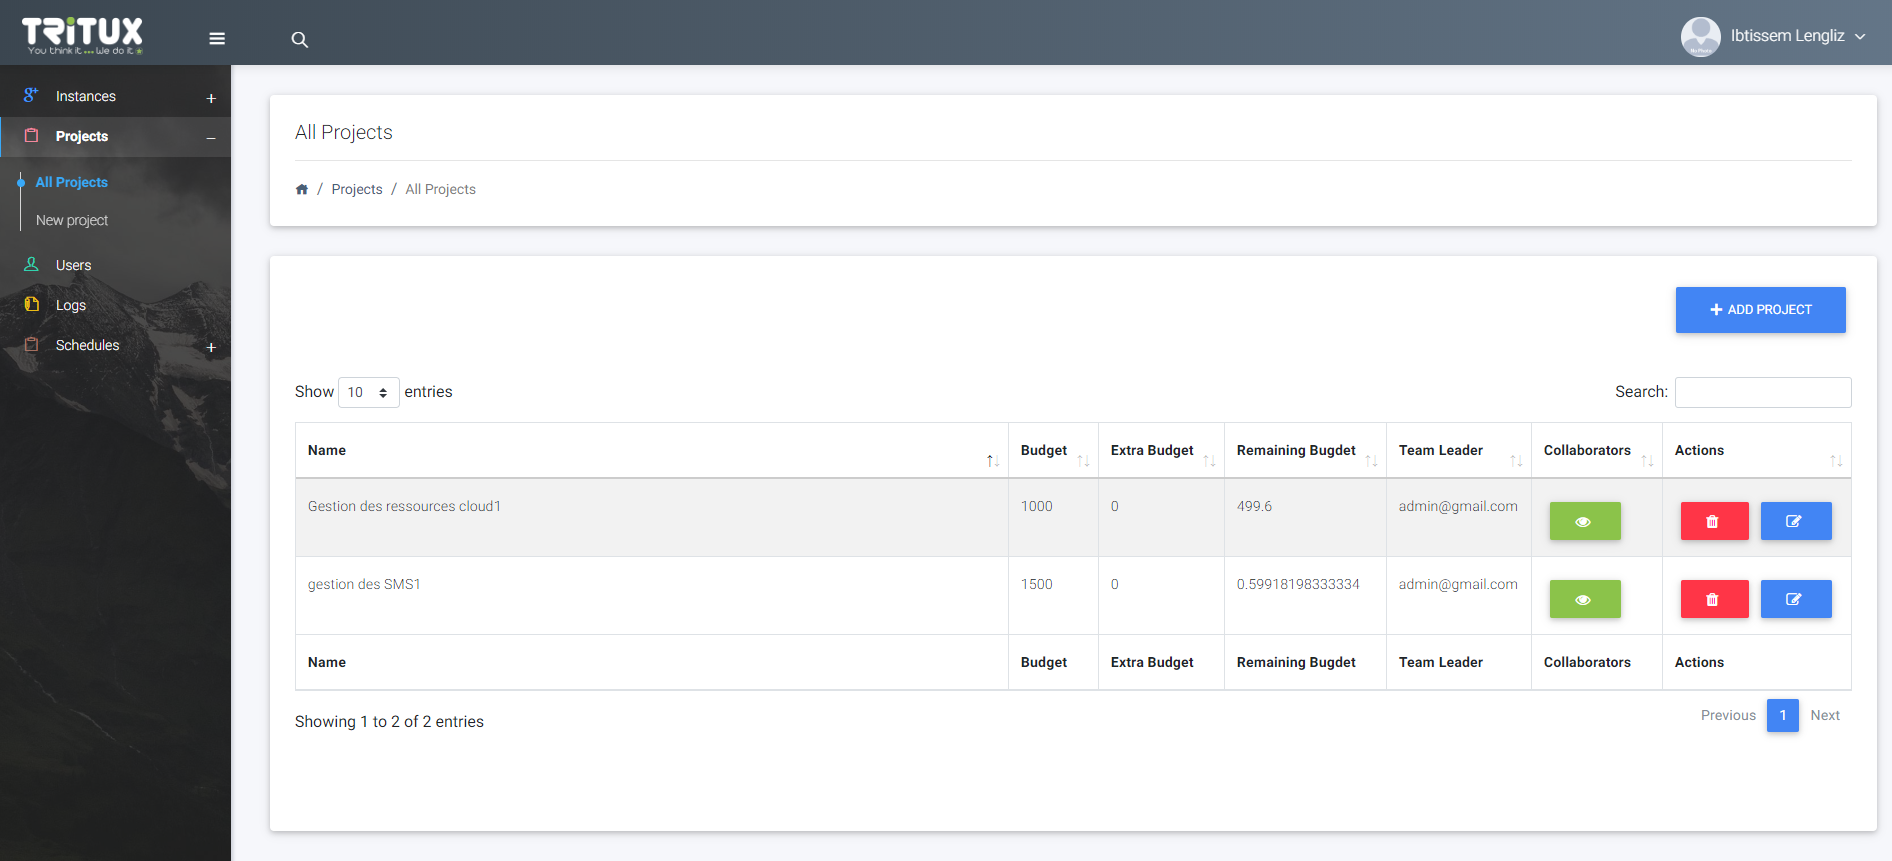
\includegraphics[scale=0.35]{projets.PNG}
	\caption{Interface de gestion des projets}
	\label{Interface de gestion des projets}
\end{figure}

La figure 4.8 représente l'interface de gestion des projets, grâce à laquelle l'administrateur
pourra rechercher , supprimer , modifier un projet et  créer un nouveau projet comme le montre la figure 4.9 ci-dessous. 
	\begin{figure}[H]
	\centering
	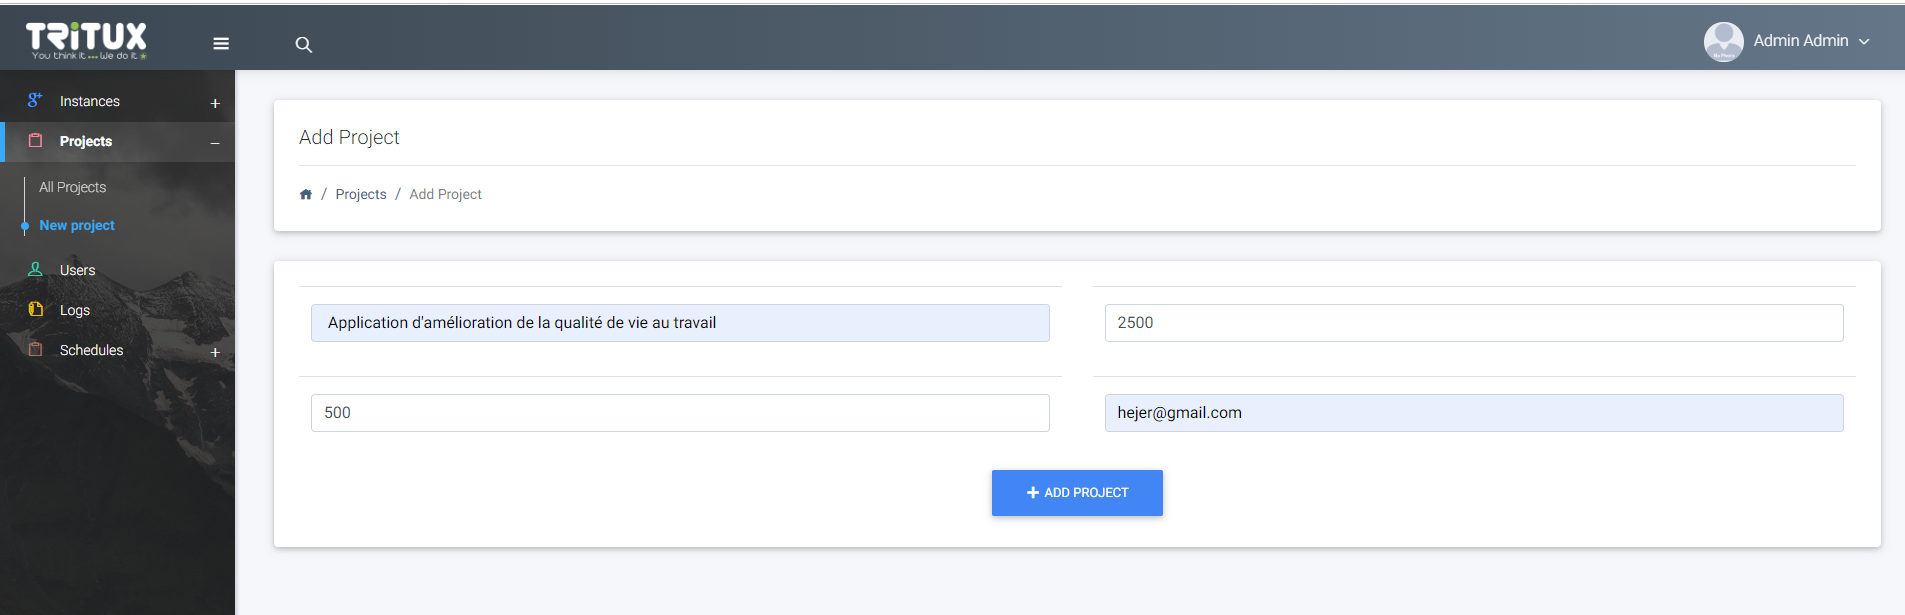
\includegraphics[scale=0.35]{addproject.PNG}
	\caption{Interface de création d'un nouveau projet}
	\label{Interface de création d'un nouveau projet}
\end{figure}

	\begin{figure}[H]
	\centering
	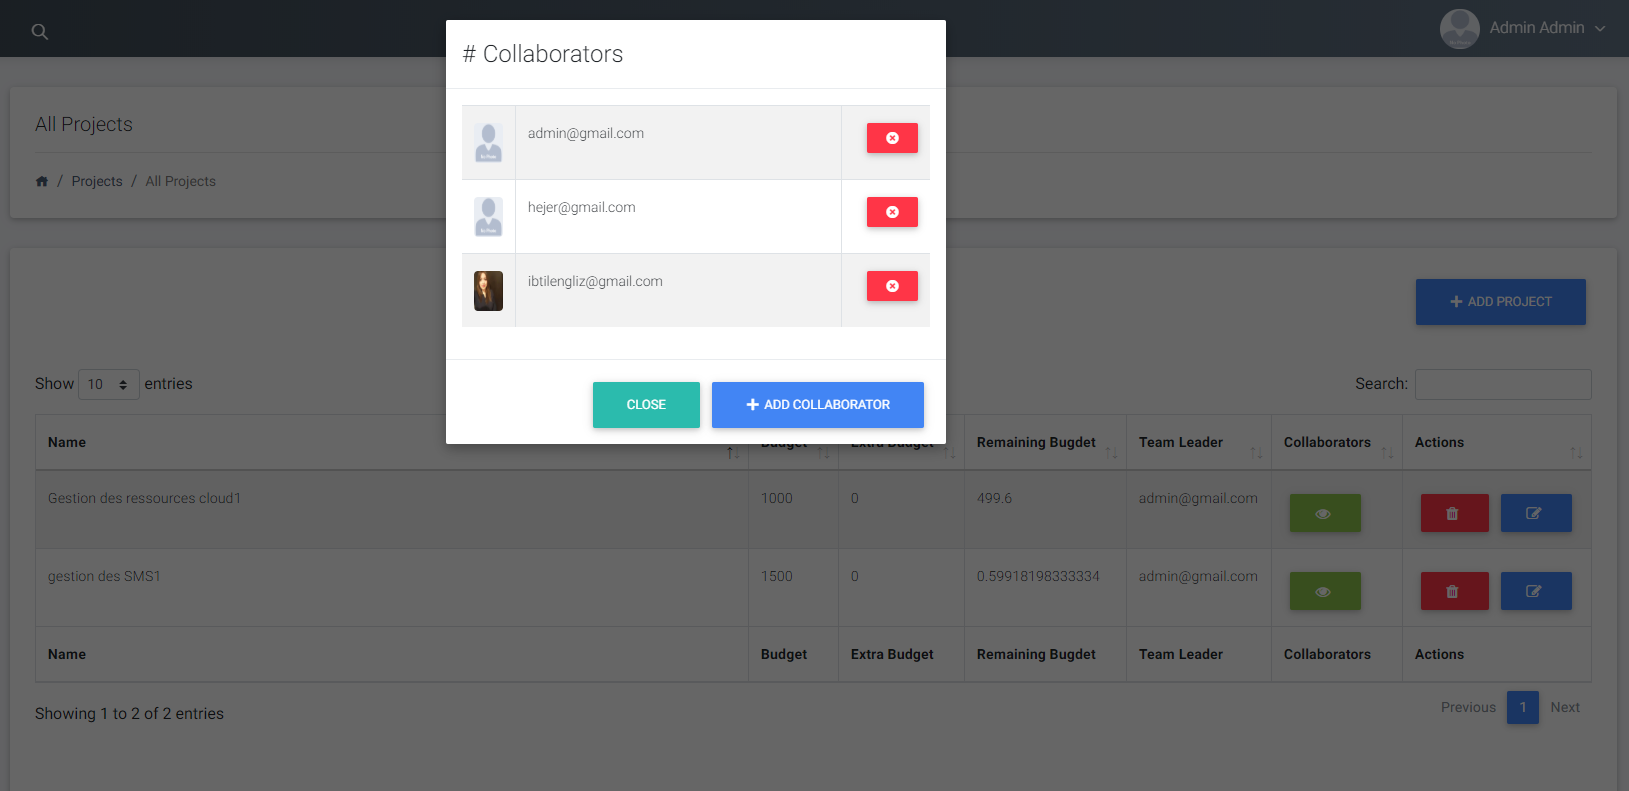
\includegraphics[scale=0.35]{membreProjets.PNG}
	\caption{Interface de gestion des membres du projet}
	\label{Interface de gestion des membres du projet}
\end{figure}
La figure 4.10 ci dessus met en évidence la gestion des membres du projet. Dedans, le team leader peut affecter ou retirer des collaborateurs.
\begin{figure}[H]
	\centering
	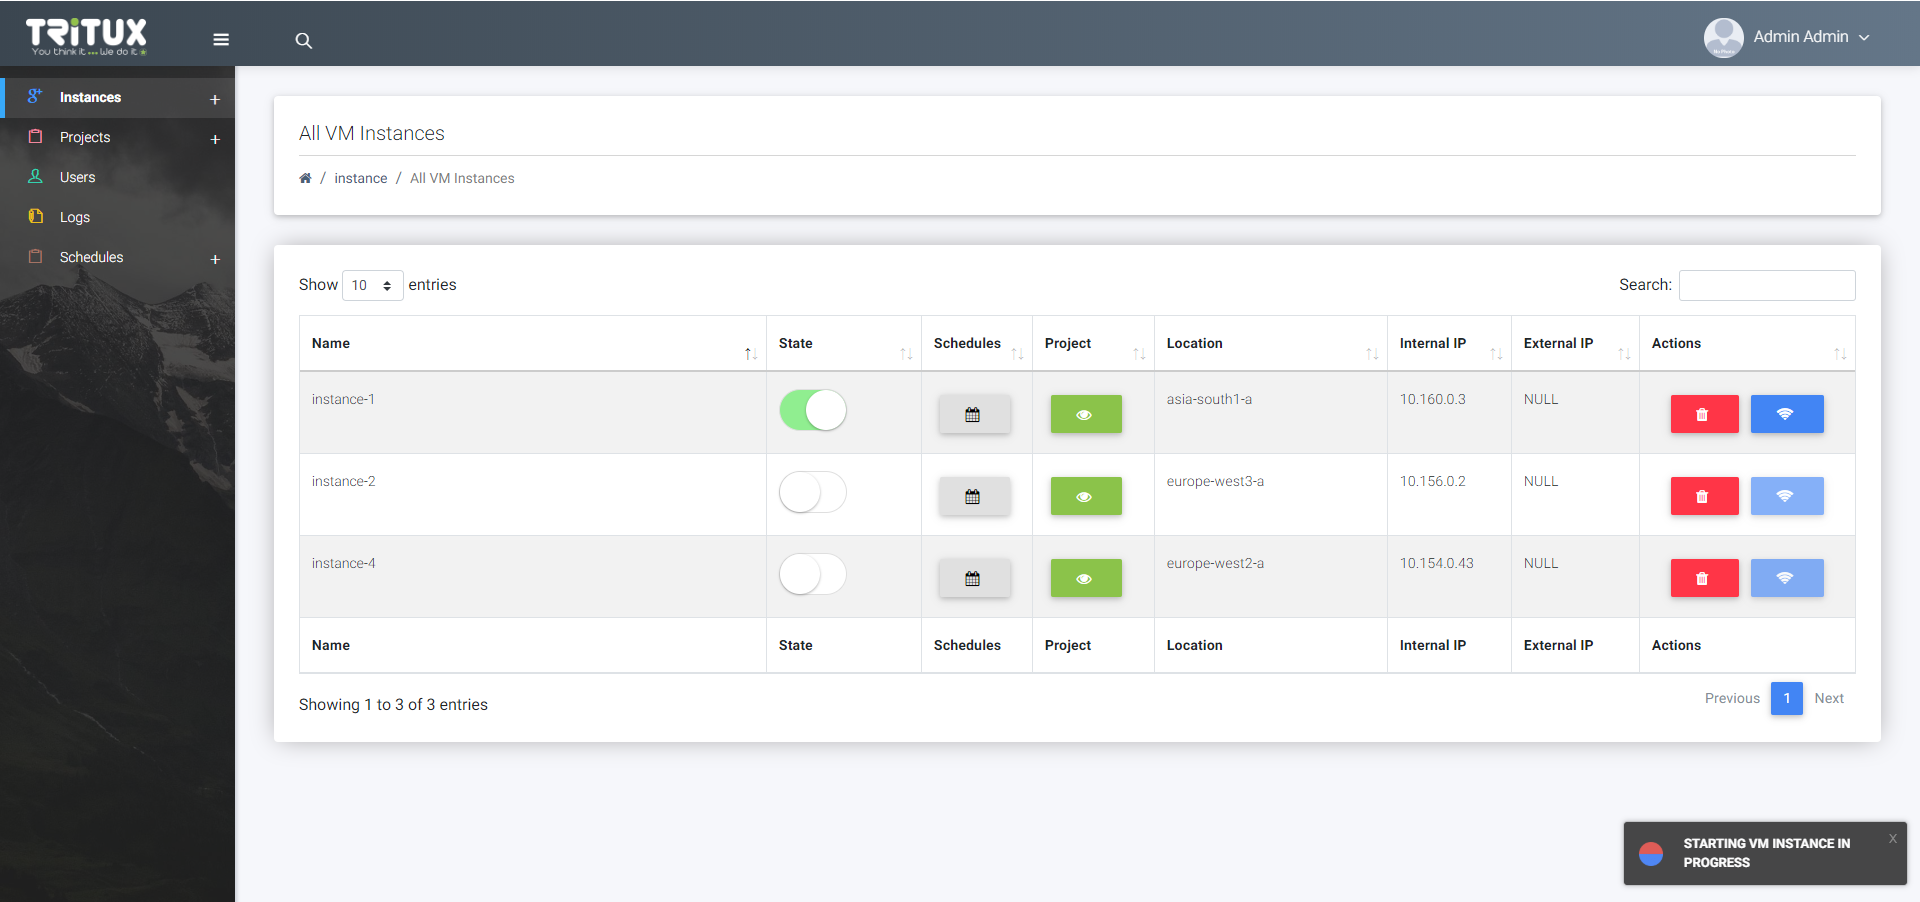
\includegraphics[scale=0.273]{instances.png}
	\caption{Interface de gestion des instances de machine virtuelle}
	\label{Interface de gestion des instances de machine virtuelle}
\end{figure}

La figure 4.11 représente l'interface de gestion des machines virtuelles, grâce à laquelle l'administrateur
pourra rechercher , supprimer , orchestrer le fonctionnement des VMs , affecter un planning, modifier le projet de chaque VM et créer une machine virtuelle comme le montre la figure 4.12. 
Ce dernier il peut aussi consulter les détails de chaque instance de machine virtuelle grâce à la figure 4.13.

\begin{figure}[H]
	\centering
	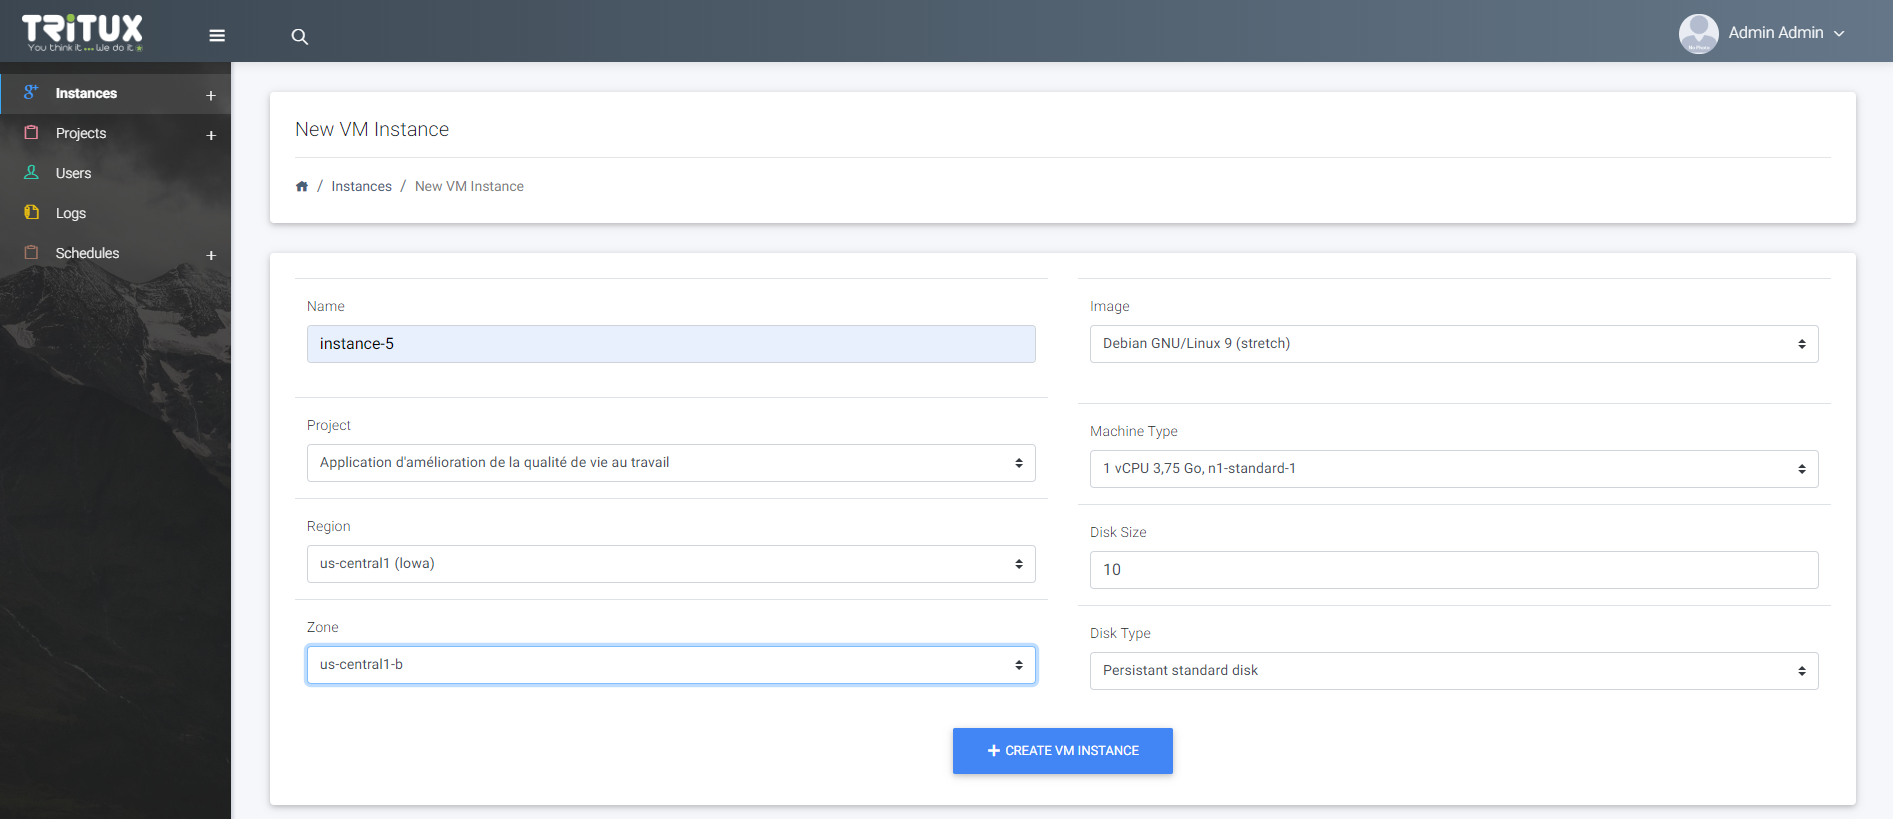
\includegraphics[scale=0.35]{createvm.png}
	\caption{Interface de création d'une nouvelle instance de machine virtuelle}
	\label{Interface de création d'une nouvelle instance de machine virtuelle}
\end{figure}
\begin{figure}[H]
	\centering
	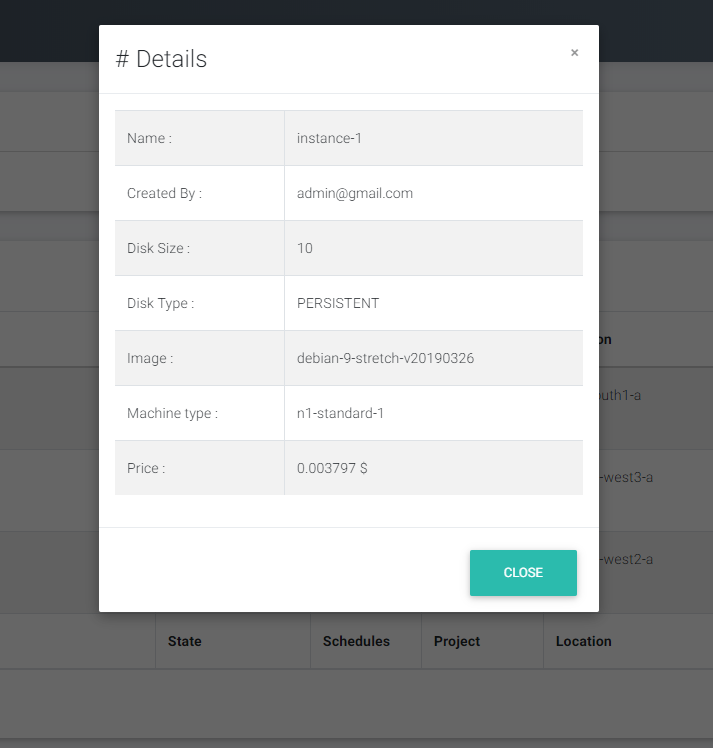
\includegraphics[scale=0.35]{details.PNG}
	\caption{Interface de détails des instances de machine virtuelle}
	\label{Interface des détails des instances de machine virtuelle}
\end{figure}

\section{Conclusion}
Au cours de ce sprint nous avons pu détaillé les principaux fonctionnalités  de la partie la plus importante de notre application qui est la gestion des machines virtuelle et des projets. Cette partie met en évidence la contrôle des VMs par projet et son budget. Dans le
chapitre suivant nous allons attaquer avec la même approche le troisième sprint.